%!TEX root = report.tex
\subsection{Image Processing}
\label{sec:imageprocessing}

The implemented procedure to detect the image of the robot head and the reference points is based on bright colored, circular reference points and is semi-automatic.

Examining the picture's HSV representation (Figures \ref{fig:img_h} and \ref{fig:img_s}), one can see that a combination of the H and S values gives a good criteria for the extraction of the bright colored points. 
The user defines the regions of interest and the relative position of the reference points by clicking in order on these points in the order of their numbering.
The colors in these regions of interest are extracted in two steps: first a rough filter is applied to the image which filters out any pixels that lie outside of a certain color range and sets their values to 0 (Figures. 
The color distribution of the left over pixels is then characterized by its mean $\mu$ and standard deviation $\sigma$ and only colors lying above and below a certain threshold are preserved. Formally the criterion for pixels that are kept is:

\begin{equation}
    \frac{I(x,y)-\mu}{\sigma}\leq z
\end{equation}

The threshold $z$ is empirically chosen to be 2, which, if the colorspectrum had the form of a gaussian, would correspond to keeping around 99\% of the colors.
The contours of the resulting binary image undergo two tests. 
%TODO Explain how contours are found
First, the area within the contour has to lie above a empirically found minimum for the contour to be further treated. The resulting contours are shown and the regions of interest are shown in Figure \ref{fig:img_org}. 
Secondly, the circular shape is tested by placing a circular filter of an approximate radius onto the contours and counting the white pixels that lie inside the circle and outside the circle respectively (true positives and false positives). 
The proportion of true positives has to lie above a certain threshold $t$ for the contour to be considered valid.  
The resulting binary image is composed of at least $N_{pts}$ contours whose centroids can be obtained by calculating the respective moments $M_{i,j}=\sum_{x} \sum_{y} x^iy^i I(x,y)$ ($x$ and $y$ correspond to pixel coordinates and $I(x,y)$ is the pixel intensity). 
The centroid coordinates are given by $\bar{x}=\frac{M_{10}}{M_{00}}$ and $\bar{y}=\frac{M_{01}}{M_{00}}$. If two centroids are too close to each other, they are considered a duplicate and repliced by their middle.
The resulting binary images with the final centroids for each point for reference points and the robot head are shown in Figures \ref{fig:circ_org} and \ref{fig:circ_red} respectively.
\begin{figure}[H]
	\centering
	\begin{subfigure}[b]{0.49\linewidth}
        \centering
		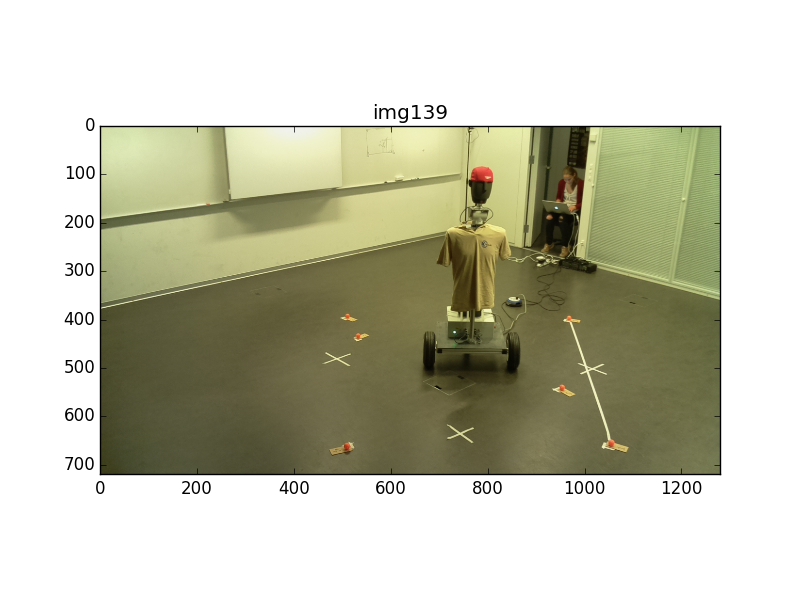
\includegraphics[width=\linewidth]{files/_img139_cvt.png}
		\caption{original image}
		\label{fig:img}
	\end{subfigure}
	\begin{subfigure}[b]{0.49\linewidth}
        \centering
		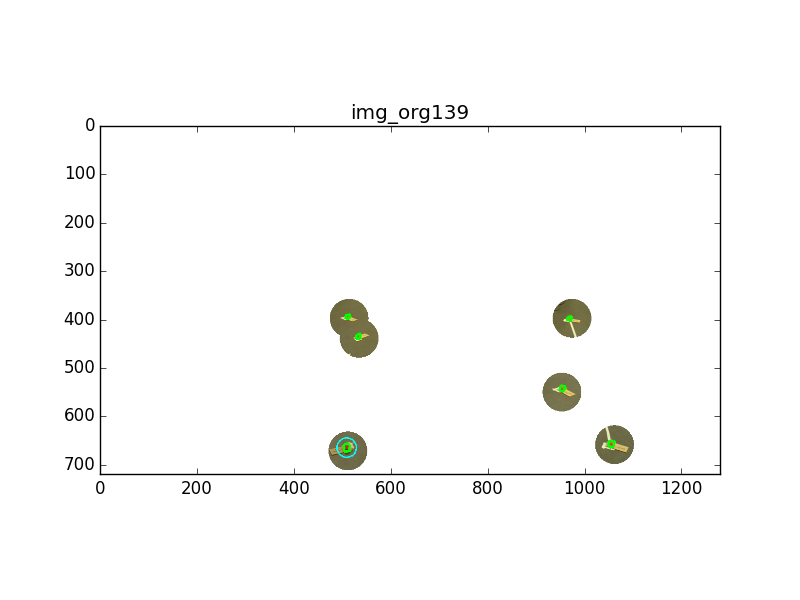
\includegraphics[width=\linewidth]{files/_img_org139.png}
		\caption{Regions of interest and extracted colors}
		\label{fig:img_org}
	\end{subfigure}
	\begin{subfigure}[b]{0.49\linewidth}
        \centering
		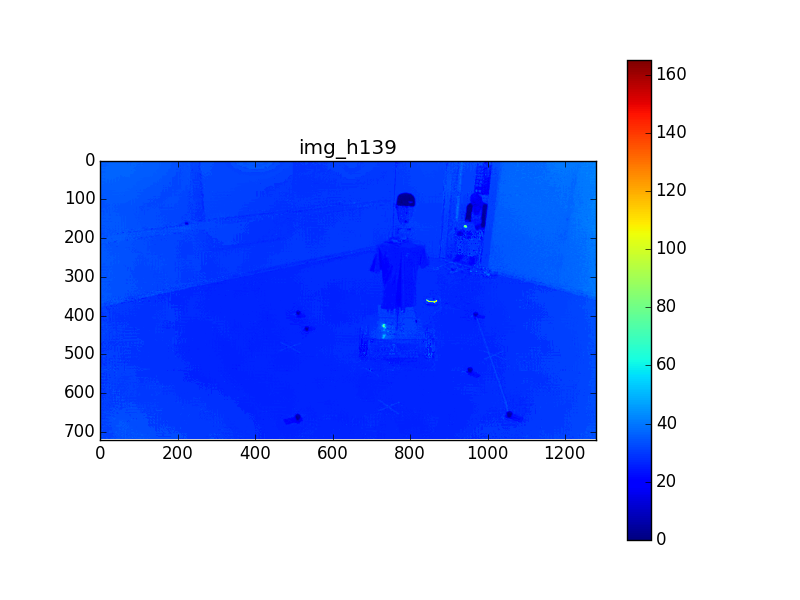
\includegraphics[width=\linewidth]{files/_img_h139.png}
		\caption{\textbf{Hue} representation of original image}
		\label{fig:img_h}
	\end{subfigure}
	\begin{subfigure}[b]{0.49\linewidth}
        \centering
		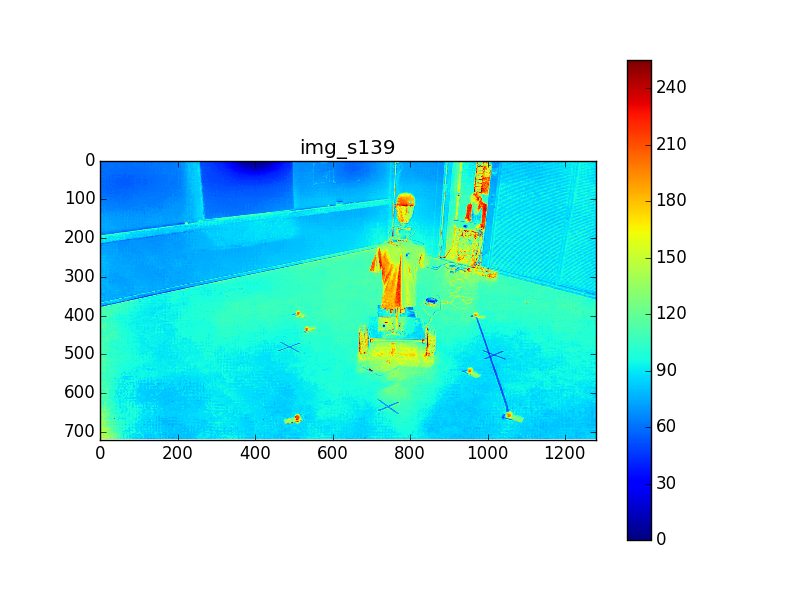
\includegraphics[width=\linewidth]{files/_img_s139.png}
		\caption{\textbf{Saturation} representation of original image}
		\label{fig:img_s}
	\end{subfigure}
	\begin{subfigure}[b]{0.49\linewidth}
        \centering
		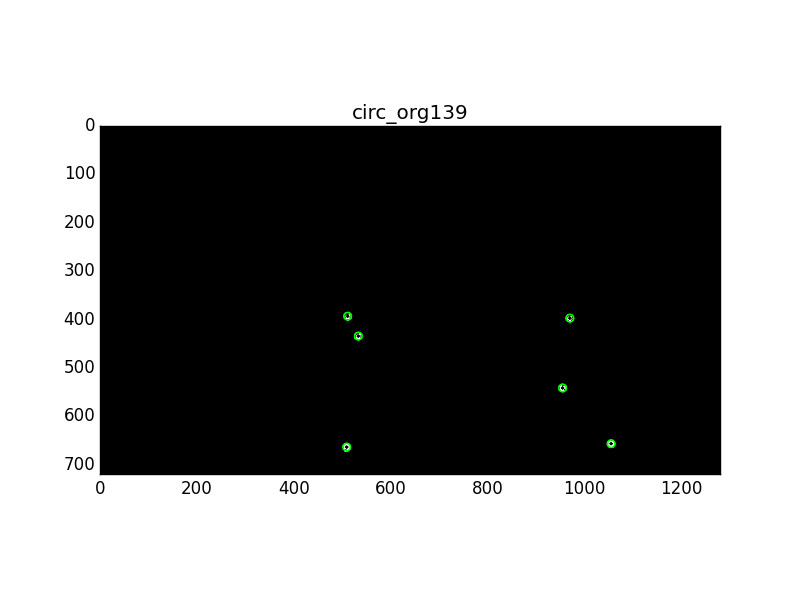
\includegraphics[width=\linewidth]{files/_circ_org139.png}
		\caption{Extracted colours, reference points}
		\label{fig:circ_org}
	\end{subfigure}
	\begin{subfigure}[b]{0.49\linewidth}
        \centering
		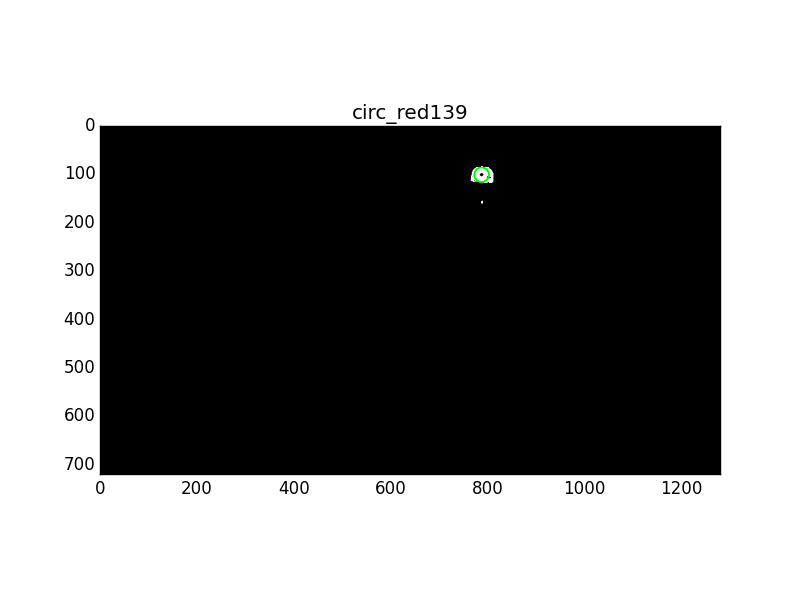
\includegraphics[width=\linewidth]{files/_circ_red139.png}
		\caption{Extracted colours, robot head}
		\label{fig:circ_red}
	\end{subfigure}
	\caption{Procedure and tools for feature extraction} 
\end{figure}

%\begin{lstlisting}[caption=Listing]
%\end{lstlisting}

